\chapter{Ogólny opis rozwiązania}
\label{cha:opis}

\section{Cel projektu}
\label{sec:celProjektu}

Celem projektu jest stworzenie aplikacji internetowej dodającej do tradycyjnych map dodatkowego wymiaru, czasu. Powinna dostarczać możliwości obserwowania zmian zachodzących na określonym terenie w danym okresie. Dodana oś czasu będzie miała za zadanie kontrolowanie okresu dla którego widoczne będą dane. Dostarczone dane przez użytkownika będą przedstawiane jemu w czytelny i umożliwiający szybką analizę sposób. Przykładowe dane wejściowe to zmiany terytorialne w przeszłości, ukazanie rozowuju miast. Końcowa wizualizacja danych oprócz prostych kształtów geometrycznych musi zapewniać obsłógę zewnętrznych plików graficznych jak i najnowszych rozwiązań służących do obsługi grafiki.

\section{Problemy do rozwiązania}
\label{sec:problemy}

\begin{itemize}

\item
Przechowywanie i transmisja danych

test

\item
Wizualizacja

Szeroki zakres informacji który może opisywać mapę musi być odpowiednio wyświetlany, w sposób czytelny i ułatwiający analizę dużych zbiorów danych.

\item
Bezpieczeństwo

Dane dostarczane przez zewnętrzny serwer powinny być wiarygodne. Użytkonwik posiadający kopię pliku znajdującą się na dysku lokalnym z infromacjami o mapię musi mieć możwliwość sprawdzenia jej autentyczności z aktualną wersją na serwerze.

\item
Optymalizacja rozwiązania

test

\end{itemize}

\section{Użytkownicy}
\label{sec:uzytkownicy}

\begin{itemize}
\item
Administrator

Osoba która posiada dostęp do serwera na krórym działa aplikacja korzystająca z omawianego frameworku. Ponieważ tworzony program jest jedynie narzędziem służącym do pracy z interaktywnymi mapami, a jednym z założeń jest jak największa adaptabliność i mozliwość działania na różnych środowiskach wymagana jest osoba która doda do działającej strony aplikację.
\item
Moderator

Pzygotowanie i edycja map powinna być wykonana przez uprawnione osoby. Może to być na przykład osoba posiadającą dużą wiedzę na dany temat, posiada ona możliwość edycji mapy.
\item
Uczeń

Użytkownik z najmniejszymy uprawnieniami, jedynie do przeglądania mapy.
\end{itemize}

\section{Granice systemu}
\label{sec:granicesystemu}

System umożliwia moderatorowi:
\begin{itemize}
\item
Tworzenie i edycję zestawów danych przechowywanych w bazie danych 

\end{itemize}

System umożliwia uczniowi:
\begin{itemize}
\item
Przeglądanie gotowych map

\item
Pracę bez konieczności stałego dostępu do internetu.
\end{itemize}

System nie umożliwia:
\begin{itemize}
\item
Wykorzystywania plików video

\end{itemize}

\section{Lista możliwości}
\label{sec:listamozliwosci}

Praca z mapami w trybie offline
\begin{itemize}
\item
wczytywanie plików

\item
przechywanie danych po stornie klienta

\item


\end{itemize}

Szeroki wachlarz dostęnych sposobów wizualizacji danych
\begin{itemize}
\item
Korzystanie z grafiki wektorowej

\item
współpraca z plikami graficznymi

\item
obśługa animacji poprzez svg

\item
aproksymacja danych

\end{itemize}

Współpraca z zewętrznymi aplikacjami
\begin{itemize}
\item
obłsuga plików xklllll

\item
parsowanie danych z formatu xml to pamięci storage
\end{itemize}

Tworzenie interaktywnych filtów
\begin{itemize}
\item
filtry obsługjące zminę czasu 

\item
filtry obsługujące zmianę mapy

\end{itemize}

\section{Specyfikacja wymagań}
\label{sec:specyfikacja wymagan}

\subsection{Ogólny diagram przypadków użycia}

\label{sec:diagramcaseuse}
\begin{figure}[H]
  \centering
    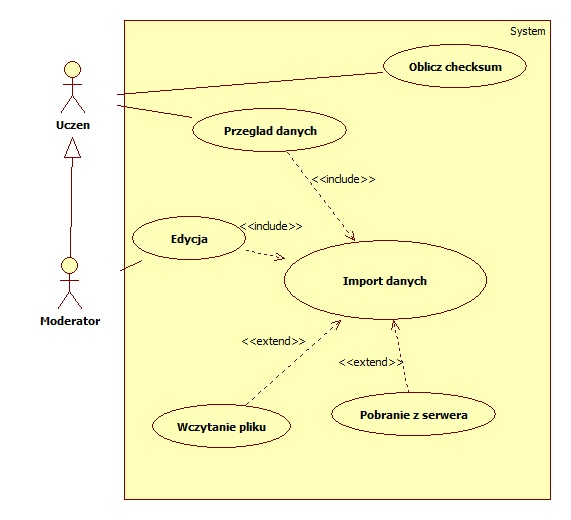
\includegraphics[width=\textwidth]{ge/caseuse.jpg}
  \caption{Case use.}
  \label{fig:caseuse}
\end{figure}

\subsection{Definicje przypadków użycia}
\label{sec:defCaseuse}

\begin{table}[H]
    \centering
    \begin{tabular}{|l|l|}
    \hline
    Nazwa przypadku użycia & fggg  \\ \hline
    Typ przypadku użycia  & Ogólny  \\ \hline
    Aktorzy   & ~     \\ \hline
    Warunki wstępne   & ~     \\ \hline
    Warunku końcowe dla sukcesu   & ~     \\ \hline
    Warunki końcowe dla niepowodzenia   & ~     \\ \hline
    Scenariusz główny   & ~     \\ \hline
    Scenariusz alternatywny   & ~     \\ \hline
    \end{tabular}
    \caption{Przypadek ...}
    \label{tab:caseuse1}
\end{table}

\begin{table}[H]
    \centering
    \begin{tabular}{|l|l|}
    \hline
    Nazwa przypadku użycia & fggg  \\ \hline
    Typ przypadku użycia  & Ogólny  \\ \hline
    Aktorzy   & ~     \\ \hline
    Warunki wstępne   & ~     \\ \hline
    Warunku końcowe dla sukcesu   & ~     \\ \hline
    Warunki końcowe dla niepowodzenia   & ~     \\ \hline
    Scenariusz główny   & ~     \\ \hline
    Scenariusz alternatywny   & ~     \\ \hline
    \end{tabular}
    \caption{Przypadek 2...}
    \label{tab:caseuse2}
\end{table}

\begin{table}[H]
    \centering
    \begin{tabular}{|l|l|}
    \hline
    Nazwa przypadku użycia & fggg  \\ \hline
    Typ przypadku użycia  & Ogólny  \\ \hline
    Aktorzy   & ~     \\ \hline
    Warunki wstępne   & ~     \\ \hline
    Warunku końcowe dla sukcesu   & ~     \\ \hline
    Warunki końcowe dla niepowodzenia   & ~     \\ \hline
    Scenariusz główny   & ~     \\ \hline
    Scenariusz alternatywny   & ~     \\ \hline
    \end{tabular}
    \caption{Przypadek 2...}
    \label{tab:caseuse2}
\end{table}

\subsection{Wymagania niefunkcjonalne}
\label{sec:niefunkcjonalnes}

Oprócz wymagań dotyczących prawidłowego funkcjonowania aplikacji, wymagane jest
aby zapewnione były poniższe punkty.

\begin{itemize}
\item 
The first item

\item 
System powinien być skalowalny, powinien umożliwiać dostęp wielu użytkownikom równocześnie przy zachowaniu wymagań wydajnościowych.

\item
Aplikacja powinna działać identycznie na różnych środowiskach i przeglądarkach internetowych.
\end{itemize}